\documentclass[notitlepage]{article}
\usepackage{ctex}
\usepackage{amsmath}
\usepackage{amssymb}
\usepackage{indentfirst}
\usepackage{graphicx}
\usepackage{float}
\usepackage{subfig}
\usepackage{overpic}
\usepackage[a4paper, scale=0.85]{geometry}

\title{实验二\ KNN分类任务}
\author{}
\date{}

\setlength{\parindent}{2em}
\linespread{2}

\begin{document}

\maketitle

\vspace{-7em}

\section{问题描述}

通过KNN算法对Iris鸢尾花数据集中的测试集进行分类,分别使用欧式距离以及
马氏距离作为度量实现,同时实现基于马氏距离的度量学习算法NCA

\section{实现步骤与流程}

\subsection*{KNN算法}

KNN算法选取训练集中与未见演本的度量最小的 $k$ 个样本中类别众数作为预测值

\subsection*{NCA算法}

样本的散布矩阵
\begin{equation*}
\mathbf{S} = \frac{1}{n} \sum_{i = 1}^{n} (\boldsymbol{x}_{i} - \boldsymbol{\mu}) 
(\boldsymbol{x} - \boldsymbol{\mu})^{\mathrm{T}}
\end{equation*}

马式距离
\begin{equation*}
d_{M}(\boldsymbol{x}_{i},\ \boldsymbol{x}_{j}) = 
\sqrt{(\boldsymbol{x_{i}} - \boldsymbol{x}_{j})^{\mathrm{T}} 
\mathbf{S}^{-1} (\boldsymbol{x}_{i} - \boldsymbol{x}_{j})}
\end{equation*}

可学习的马式距离(伪马式距离)
\begin{equation*}
d_{M}(\boldsymbol{x}_{i},\ \boldsymbol{x}_{j}) = 
\sqrt{(\boldsymbol{x_{i}} - \boldsymbol{x}_{j})^{\mathrm{T}} 
\mathbf{M} (\boldsymbol{x}_{i} - \boldsymbol{x}_{j})}
\end{equation*}

其中,$\mathbf{M}$ 是半正定矩阵,重写以上距离数学形式
\begin{equation*}
d_{M}(\boldsymbol{x}_{i},\ \boldsymbol{x}_{j}) = 
\sqrt{(\boldsymbol{x}_{i} - \boldsymbol{x}_{j})^{\mathrm{T}} 
\mathbf{A}^{\mathrm{T}} \mathbf{A} (\boldsymbol{x}_{i} - \boldsymbol{x}_{j})}
\end{equation*}

其中变换矩阵 $\mathbf{A} \in \mathbb{R}^{k \times d}$ ,
并且 $k \ge rank(\mathbf{M})$。设样本 $\boldsymbol{x}_{i}$ 的近邻分布为
\begin{gather*}
    p_{ij} = \exp\{-d^{2}_{M}(\boldsymbol{x}_{i},\ 
    \boldsymbol{x}_{j})\} \bigg/ Z_{i} \\ \\
    Z_{i} = \sum_{k \ne i} 
    \exp\{ -d^{2}_{M}(\boldsymbol{x}_{i},\ \boldsymbol{x}_{k}) \}
\end{gather*}

代表样本 $\boldsymbol{x}_{j}$ 与样本 $\boldsymbol{x}_{i}$ 属于相同类别的概率。
针对变换矩阵 $\mathbf{A}$ 最大化同类样本相似程度
\begin{equation*}
    \max_{\mathbf{A}} f(\mathbf{A}) = \sum_{i = 1}^{n} 
    \sum_{j \in \Omega_{i}} p_{ij}
\end{equation*}

其中 $\Omega_{i}$ 表示和样本 $\boldsymbol{x}_{i}$ 属于同一类别的其它样本的集合。令
\begin{equation*}
    d_{ij} = d^{2}_{M}(\boldsymbol{x}_{i},\ \boldsymbol{x}_{j})
\end{equation*}

准则函数对变换矩阵 $\mathbf{A}$ 求偏导数得
\begin{gather*}
    \frac{\partial p_{ij}}{\partial d_{ik}} = \left\{
    \begin{matrix}
        -p_{ij} (1 - p_{ij}) & k = j \\ \\
        p_{ij} p_{ik} & k \ne j
    \end{matrix}
    \right. \\ \\
    \frac{\partial d_{ik}}{\partial \mathbf{A}} = 
    2\mathbf{A}(\boldsymbol{x}_{i} - \boldsymbol{x}_{k}) 
    (\boldsymbol{x}_{i} - \boldsymbol{x}_{k})^{\mathrm{T}} \\ \\
    \frac{\partial p_{ij}}{\partial \mathbf{A}} = 
    2 p_{ij} \mathbf{A} \left[ \sum_{k \ne i} p_{ik} 
    (\boldsymbol{x}_{i} - \boldsymbol{x}_{k}) 
    (\boldsymbol{x}_{i} - \boldsymbol{x}_{k})^{\mathrm{T}} - 
    (\boldsymbol{x}_{i} - \boldsymbol{x}_{j}) 
    (\boldsymbol{x}_{i} - \boldsymbol{x}_{j})^{\mathrm{T}} \right]
     \\ \\
    \frac{\partial f}{\partial \mathbf{A}} = 
    \sum_{i = 1}^{n} \sum_{j \in \Omega_{i}} 
    \frac{\partial p_{ij}}{\partial \mathbf{A}}
\end{gather*}

利用梯度下降法即可学习到一个较优的变换矩阵,使得变换后的同类样本距离,异类样本远离。
但注意到该优化问题非凸,意味着最终收敛得到的解可能是局部最优解,并且与迭代初始值密切相关,
实际实验中需要多次尝试才能得到满足要求的解。

\section{实验结果与分析}

由于实验要求的MindSpore框架相关的资料较为匮乏,因此本次实验采取开源机器学习算法库
sklearn与实验中的算法进行对比。sklearn是一个开源的基于python语言的机器学习工具包。
它通过numpy, scipy等python数值计算的库实现高效的算法应用,并且涵盖了几乎所有主流机器学习算法。

\subsection*{NCA算法}

以下是NCA算法的度量学习历史以及最终收敛的模型的变换矩阵对样本进行降维后的分布图

\newpage

\begin{figure*}[htbp]
	\centering
	\subfloat[度量学习历史]{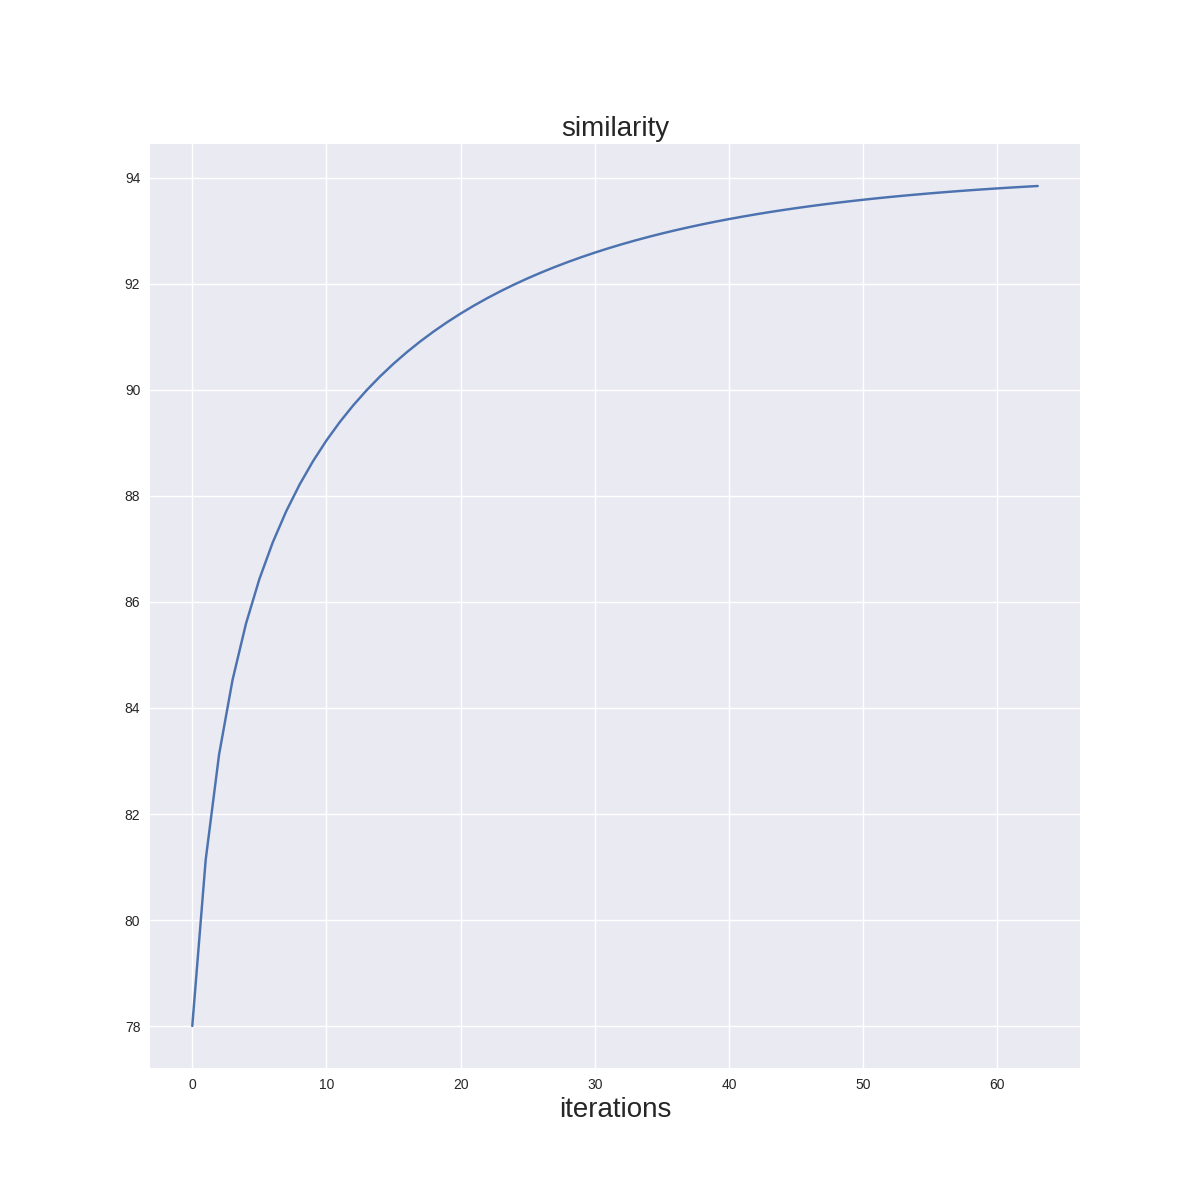
\includegraphics[width=.45\columnwidth]
    {../imgs/mine/similarity.png}}\hspace{3pt}
	\subfloat[降维样本分布]{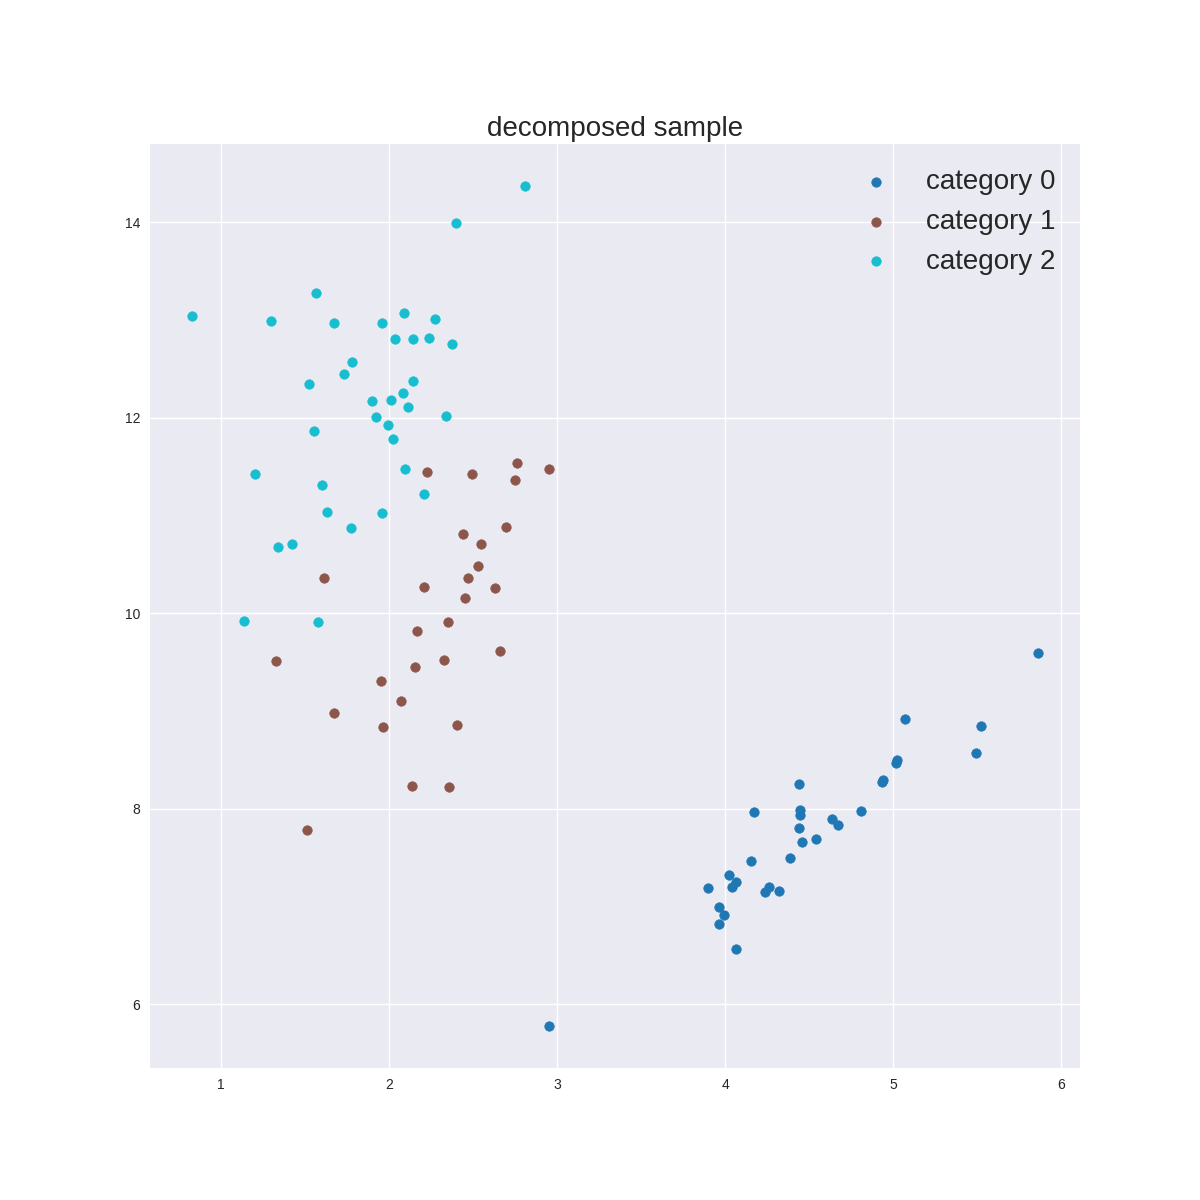
\includegraphics[width=.45\columnwidth]
    {../imgs/mine/decomposed_data.png}}
	\caption{NCA算法}
\end{figure*}

观察可得,随着模型的迭代,同类样本的相似度逐渐提高,这点也可以从降维样本上看出

\subsection*{KNN算法}

以下是实验KNN算法(欧式距离、马氏距离)与sklearn的KNN算法的在验证集上的准确率对比

\begin{figure*}[htbp]
	\centering
	\subfloat[KNN(实验)]{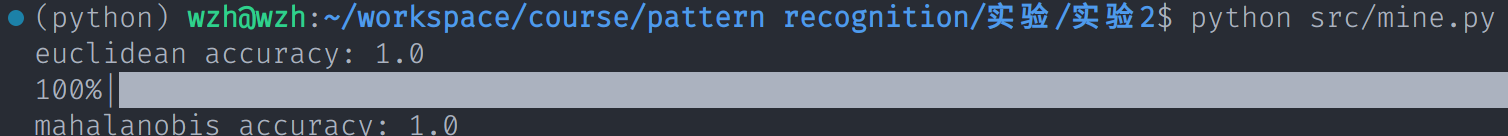
\includegraphics[width=\columnwidth]
    {../imgs/mine/acc.png}}\\
	\subfloat[KNN(sklearn)]{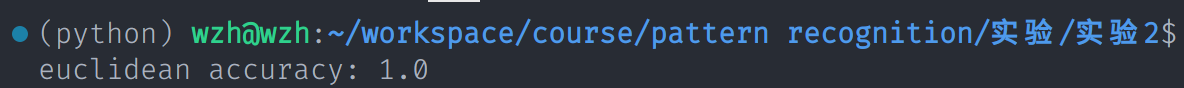
\includegraphics[width=\columnwidth]
    {../imgs/sklearn/acc.png}}
	\caption{KNN算法准确率}
\end{figure*}

经过实验,采用5近邻在验证集上可以达到最高的准确率100\%,但是由于样本数量较少,因此结果
在一定程度上作为参考

\section{MindSpore学习使用心得体会}

由于本次实验并未采用MindSpore,此部分用sklearn的学习使用心得体会来代替。

本次实验中调用了sklearn中的以下算法接口

\begin{itemize}
    \item KNN(neighbors KNeighborsClassifier)
\end{itemize}

作为实验算法的对照算法,sklearn提供的算法接口方便调用,并且执行效率较高,能够高效地实现实验的需求。

\section{代码附录}

\end{document}